\documentclass[11pt]{article}
\usepackage[margin=1in]{geometry}
\usepackage{graphicx}
\usepackage{booktabs}
\usepackage{hyperref}
\usepackage{amsmath}
\usepackage{amsfonts}
\usepackage{caption}
\usepackage{subcaption}

\title{Hybrid Music Clustering with Multi-Modal VAEs on GTZAN}
\author{CSE425 VAE Project Report}
\date{January 7, 2026}

\begin{document}
\maketitle

\begin{abstract}
We study latent representation learning for hybrid music clustering on the GTZAN dataset by integrating audio features and lyrics. We implement and compare a basic Variational Autoencoder (VAE), a Hybrid VAE (audio+lyrics), a Conditional VAE (CVAE), and Beta-VAE variants, and evaluate clustering quality with Silhouette, Calinski--Harabasz, Davies--Bouldin, Adjusted Rand Index (ARI), Normalized Mutual Information (NMI), and Purity. Across experiments, Hybrid VAE and VAE latents improve clustering over PCA baselines; Beta-VAE with moderate $\beta$ offers some disentanglement but mixed clustering gains, while CVAE shows modest improvements given limited data.
\end{abstract}

\section{Introduction}
Music genre clustering benefits from compact, semantically meaningful embeddings derived from audio and lyric modalities. Variational Autoencoders (VAEs) provide a principled framework to learn such latent spaces by maximizing the evidence lower bound (ELBO). We explore non-linear latent spaces and modality fusion to improve genre clustering quality compared to linear baselines.

\section{Related Work}
VAE~(Kingma \& Welling, 2014) formalizes deep latent-variable models trained with ELBO. Beta-VAE~(Higgins et al., 2017) scales the KL term to encourage disentanglement. CVAE~(Sohn et al., 2015) conditions the generative process on auxiliary information. For music representation, learned embeddings from audio (e.g., MFCCs, spectral features) and lyrics are widely used; clustering methods include K-Means, Agglomerative, and density-based approaches.

\section{Method}
\subsection{VAE Architecture}
Implemented in \texttt{src/models/vae.py}, our models use MLP encoders/decoders for tabular features. BasicVAE encodes audio features into a latent $z$ (e.g., hidden dims [512, 256, 128], latent dimension 128). HybridVAE employs dual encoders (audio and lyrics) to a shared latent and dual decoders for reconstruction. CVAE concatenates inputs with a one-hot genre condition. Beta-VAE scales the KL divergence by $\beta>1$.

\subsection{Objective}
We optimize the ELBO:
\begin{equation}
\mathcal{L}(x;\theta,\phi)=\mathbb{E}_{q_\phi(z|x)}[\log p_\theta(x|z)]-\beta\,\mathrm{KL}\big(q_\phi(z|x)\Vert p(z)\big),
\end{equation}
where $\beta=1$ recovers the standard VAE; $\beta>1$ yields Beta-VAE.

\subsection{Feature Extraction (Audio + Lyrics)}
Audio features (e.g., MFCCs, spectral rolloff, chroma) and lyric-derived features are combined or conditioned depending on the variant. Dataset details and EDA are in \texttt{notebooks/eda.ipynb}; raw data is under \texttt{data/GTZAN}.

\subsection{Clustering Methods}
We cluster latent vectors using K-Means and Agglomerative Clustering; in the medium track, DBSCAN is also considered. Baselines include PCA+K-Means and Autoencoder+K-Means.

\section{Experiments}
\textbf{Dataset:} GTZAN with 10 genres: blues, classical, country, disco, hiphop, jazz, metal, pop, reggae, rock. Easy track uses audio features for $\sim$609 samples; hybrid tasks use audio+lyrics for $\sim$122 samples.\\
\textbf{Preprocessing:} Standardization of features; train/eval splits where applicable; missing value checks and file existence verification.\\
\textbf{Training:} \texttt{easy/main.py}, \texttt{medium/main.py}, \texttt{hard/main.py} configure epochs (e.g., 50--150), learning rates ($5\times10^{-4}$ to $10^{-3}$), and batch sizes (e.g., 16). Latents are clustered post-training.

\section{Results}
\subsection{Easy: BasicVAE vs. PCA Baseline}
Metrics from \texttt{easy/results/metrics_comparison.csv}.
\begin{table}[h]
\centering
\caption{Easy task comparison (higher is better for Silhouette, CH, ARI, NMI, Purity; lower for Davies--Bouldin).}
\begin{tabular}{lrrrrrr}
\toprule
Method & Sil. & CH & DB & ARI & NMI & Purity \\
\midrule
VAE + K-Means & 0.2761 & 38.9772 & 1.1087 & 0.1683 & 0.4110 & 0.5082 \\
PCA + K-Means & 0.1157 & 10.4583 & 1.9604 & 0.1438 & 0.3610 & 0.4672 \\
\bottomrule
\end{tabular}
\end{table}

\begin{figure}[h]
\centering
\IfFileExists{../easy/results/vae_tsne_true.png}{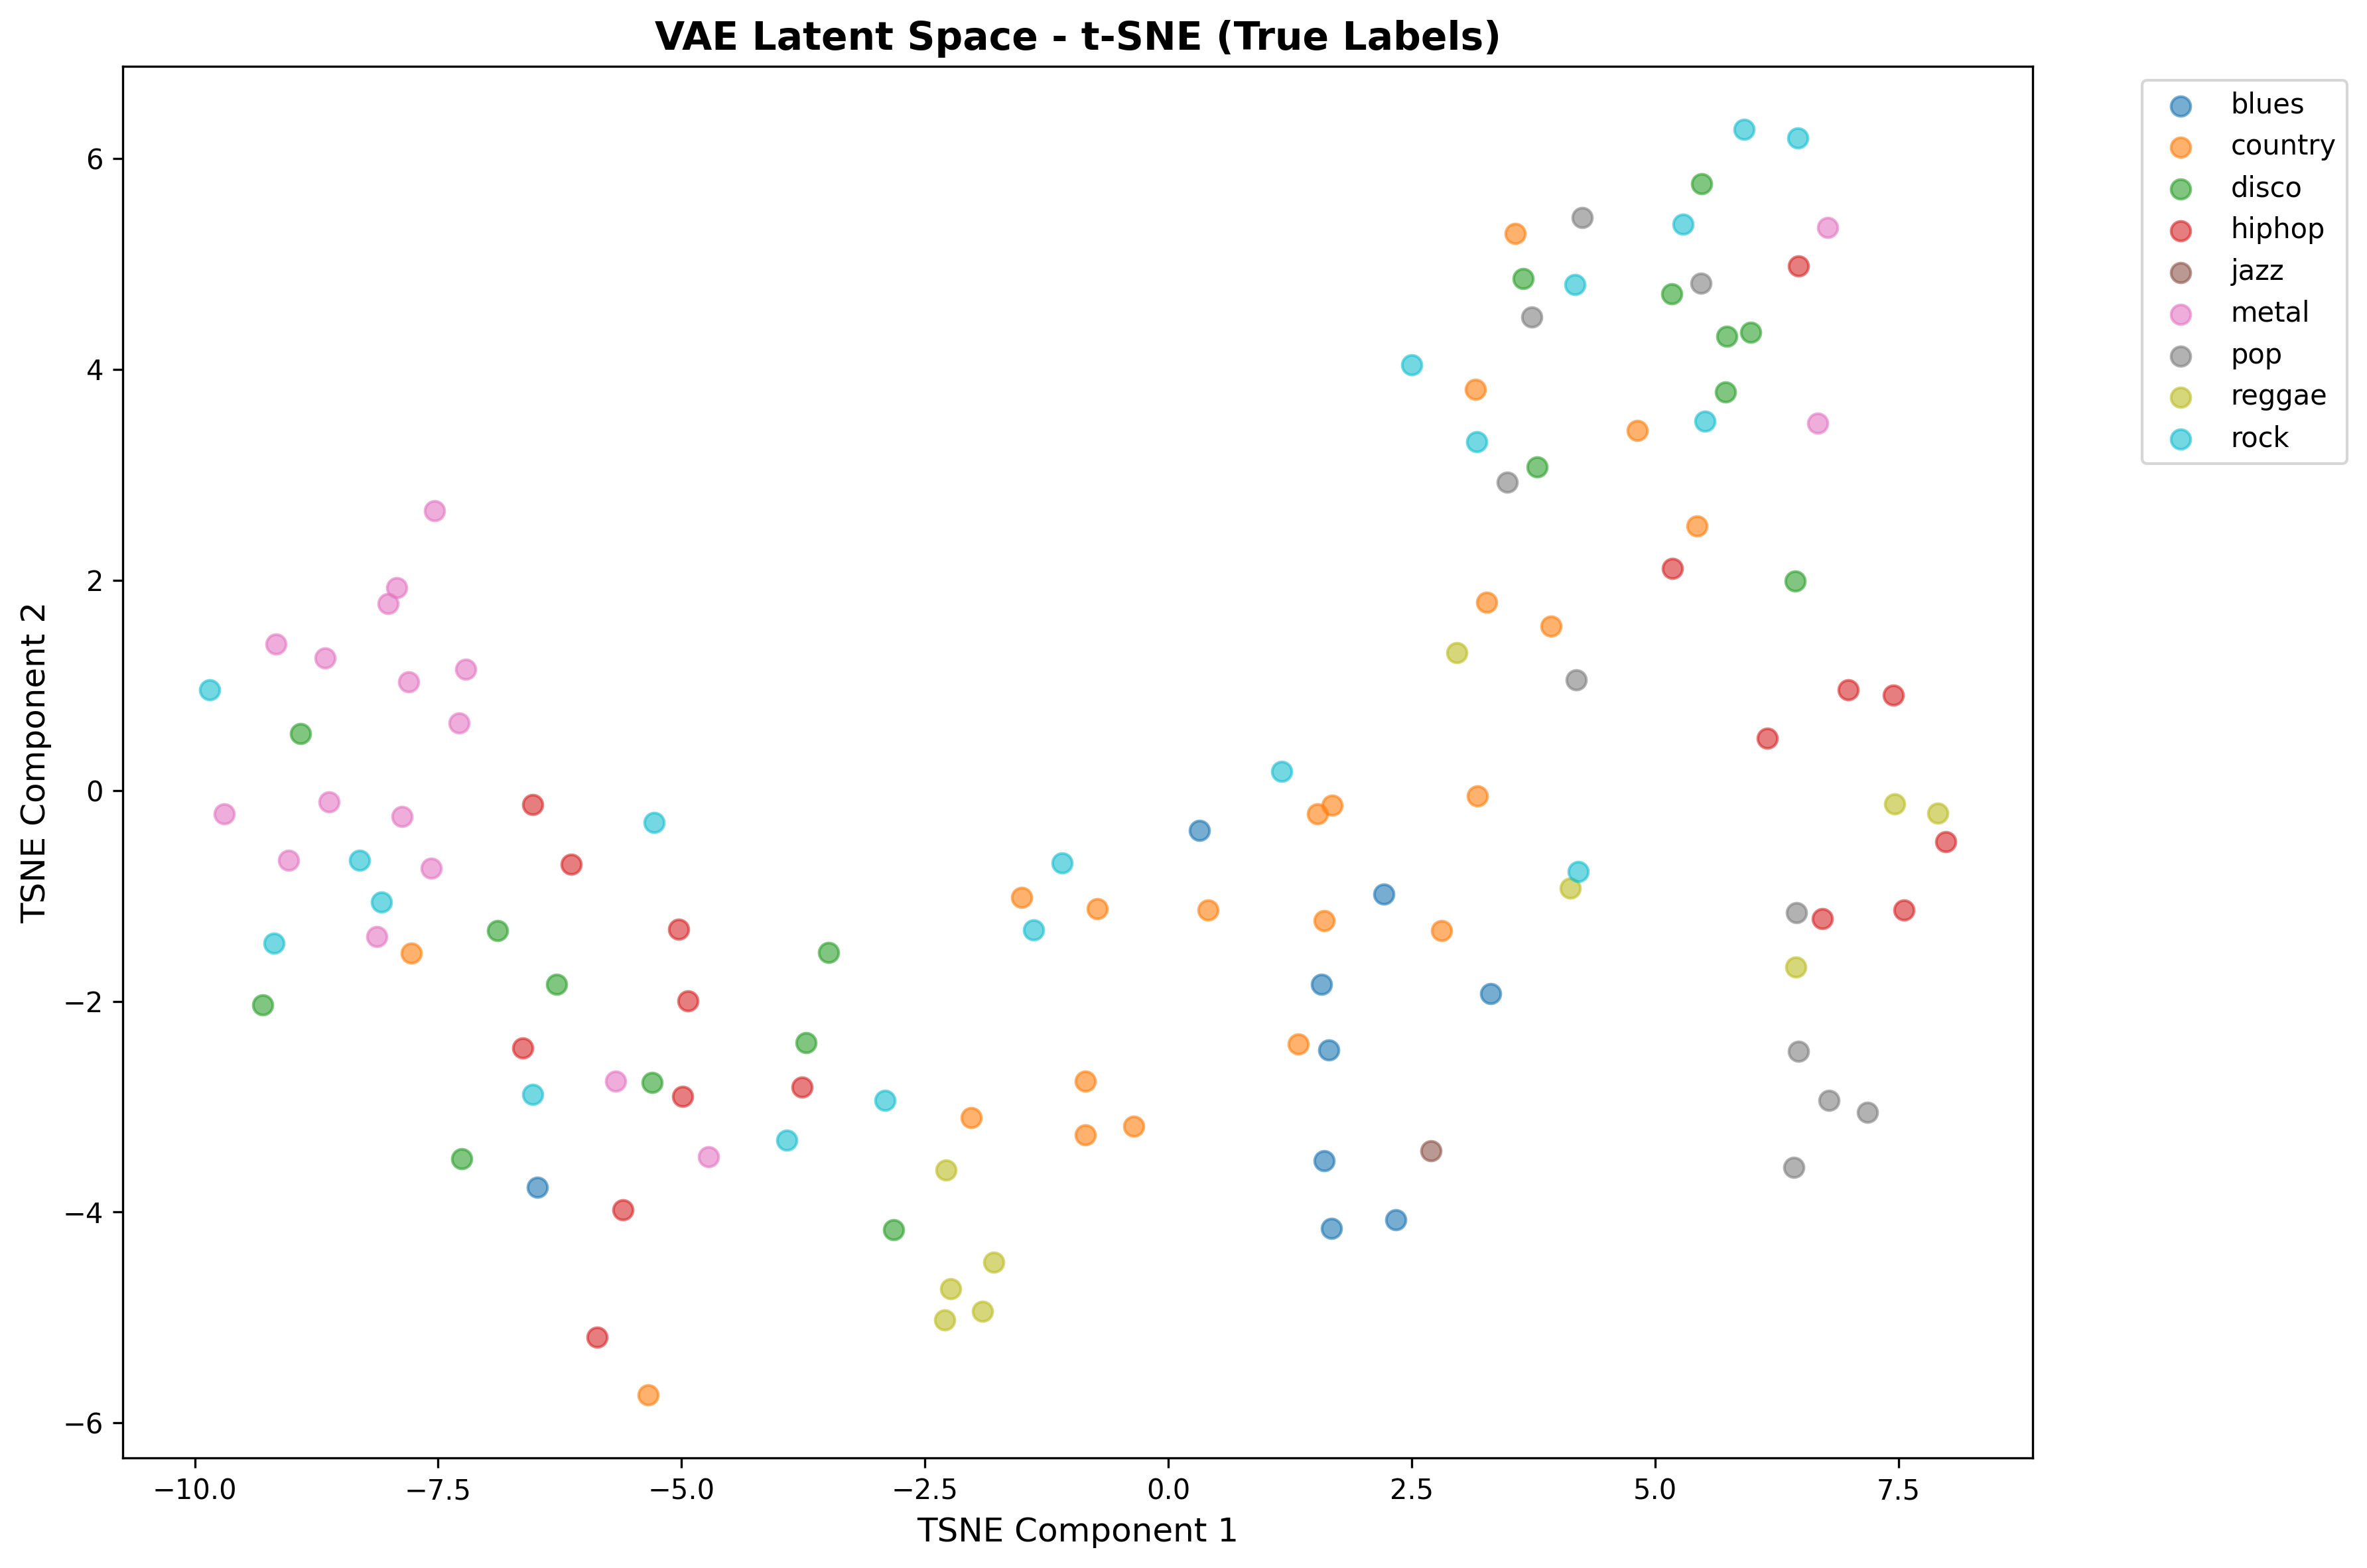
\includegraphics[width=0.9\linewidth]{../easy/results/vae_tsne_true.png}}{\fbox{Missing figure: ../easy/results/vae_tsne_true.png}}
\caption{VAE latent space t-SNE with true labels (Easy).}
\end{figure}

\subsection{Medium: HybridVAE + Multiple Clusterers}
Metrics from \texttt{medium/results/clustering_comparison.csv}.
\begin{table}[h]
\centering
\caption{Medium task comparison across clusterers.}
\begin{tabular}{lrrrrrr}
\toprule
Method & Sil. & CH & DB & ARI & NMI & Purity \\
\midrule
Agglomerative & 0.2894 & 37.6610 & 0.9001 & 0.1901 & 0.3911 & 0.4836 \\
K-Means & 0.2832 & 39.3259 & 0.9556 & 0.1888 & 0.4133 & 0.5164 \\
PCA + K-Means (Baseline) & 0.1159 & 10.4948 & 1.9605 & 0.1438 & 0.3610 & 0.4672 \\
\bottomrule
\end{tabular}
\end{table}

\begin{figure}[h]
\centering
\IfFileExists{../medium/results/hybrid_tsne_true.png}{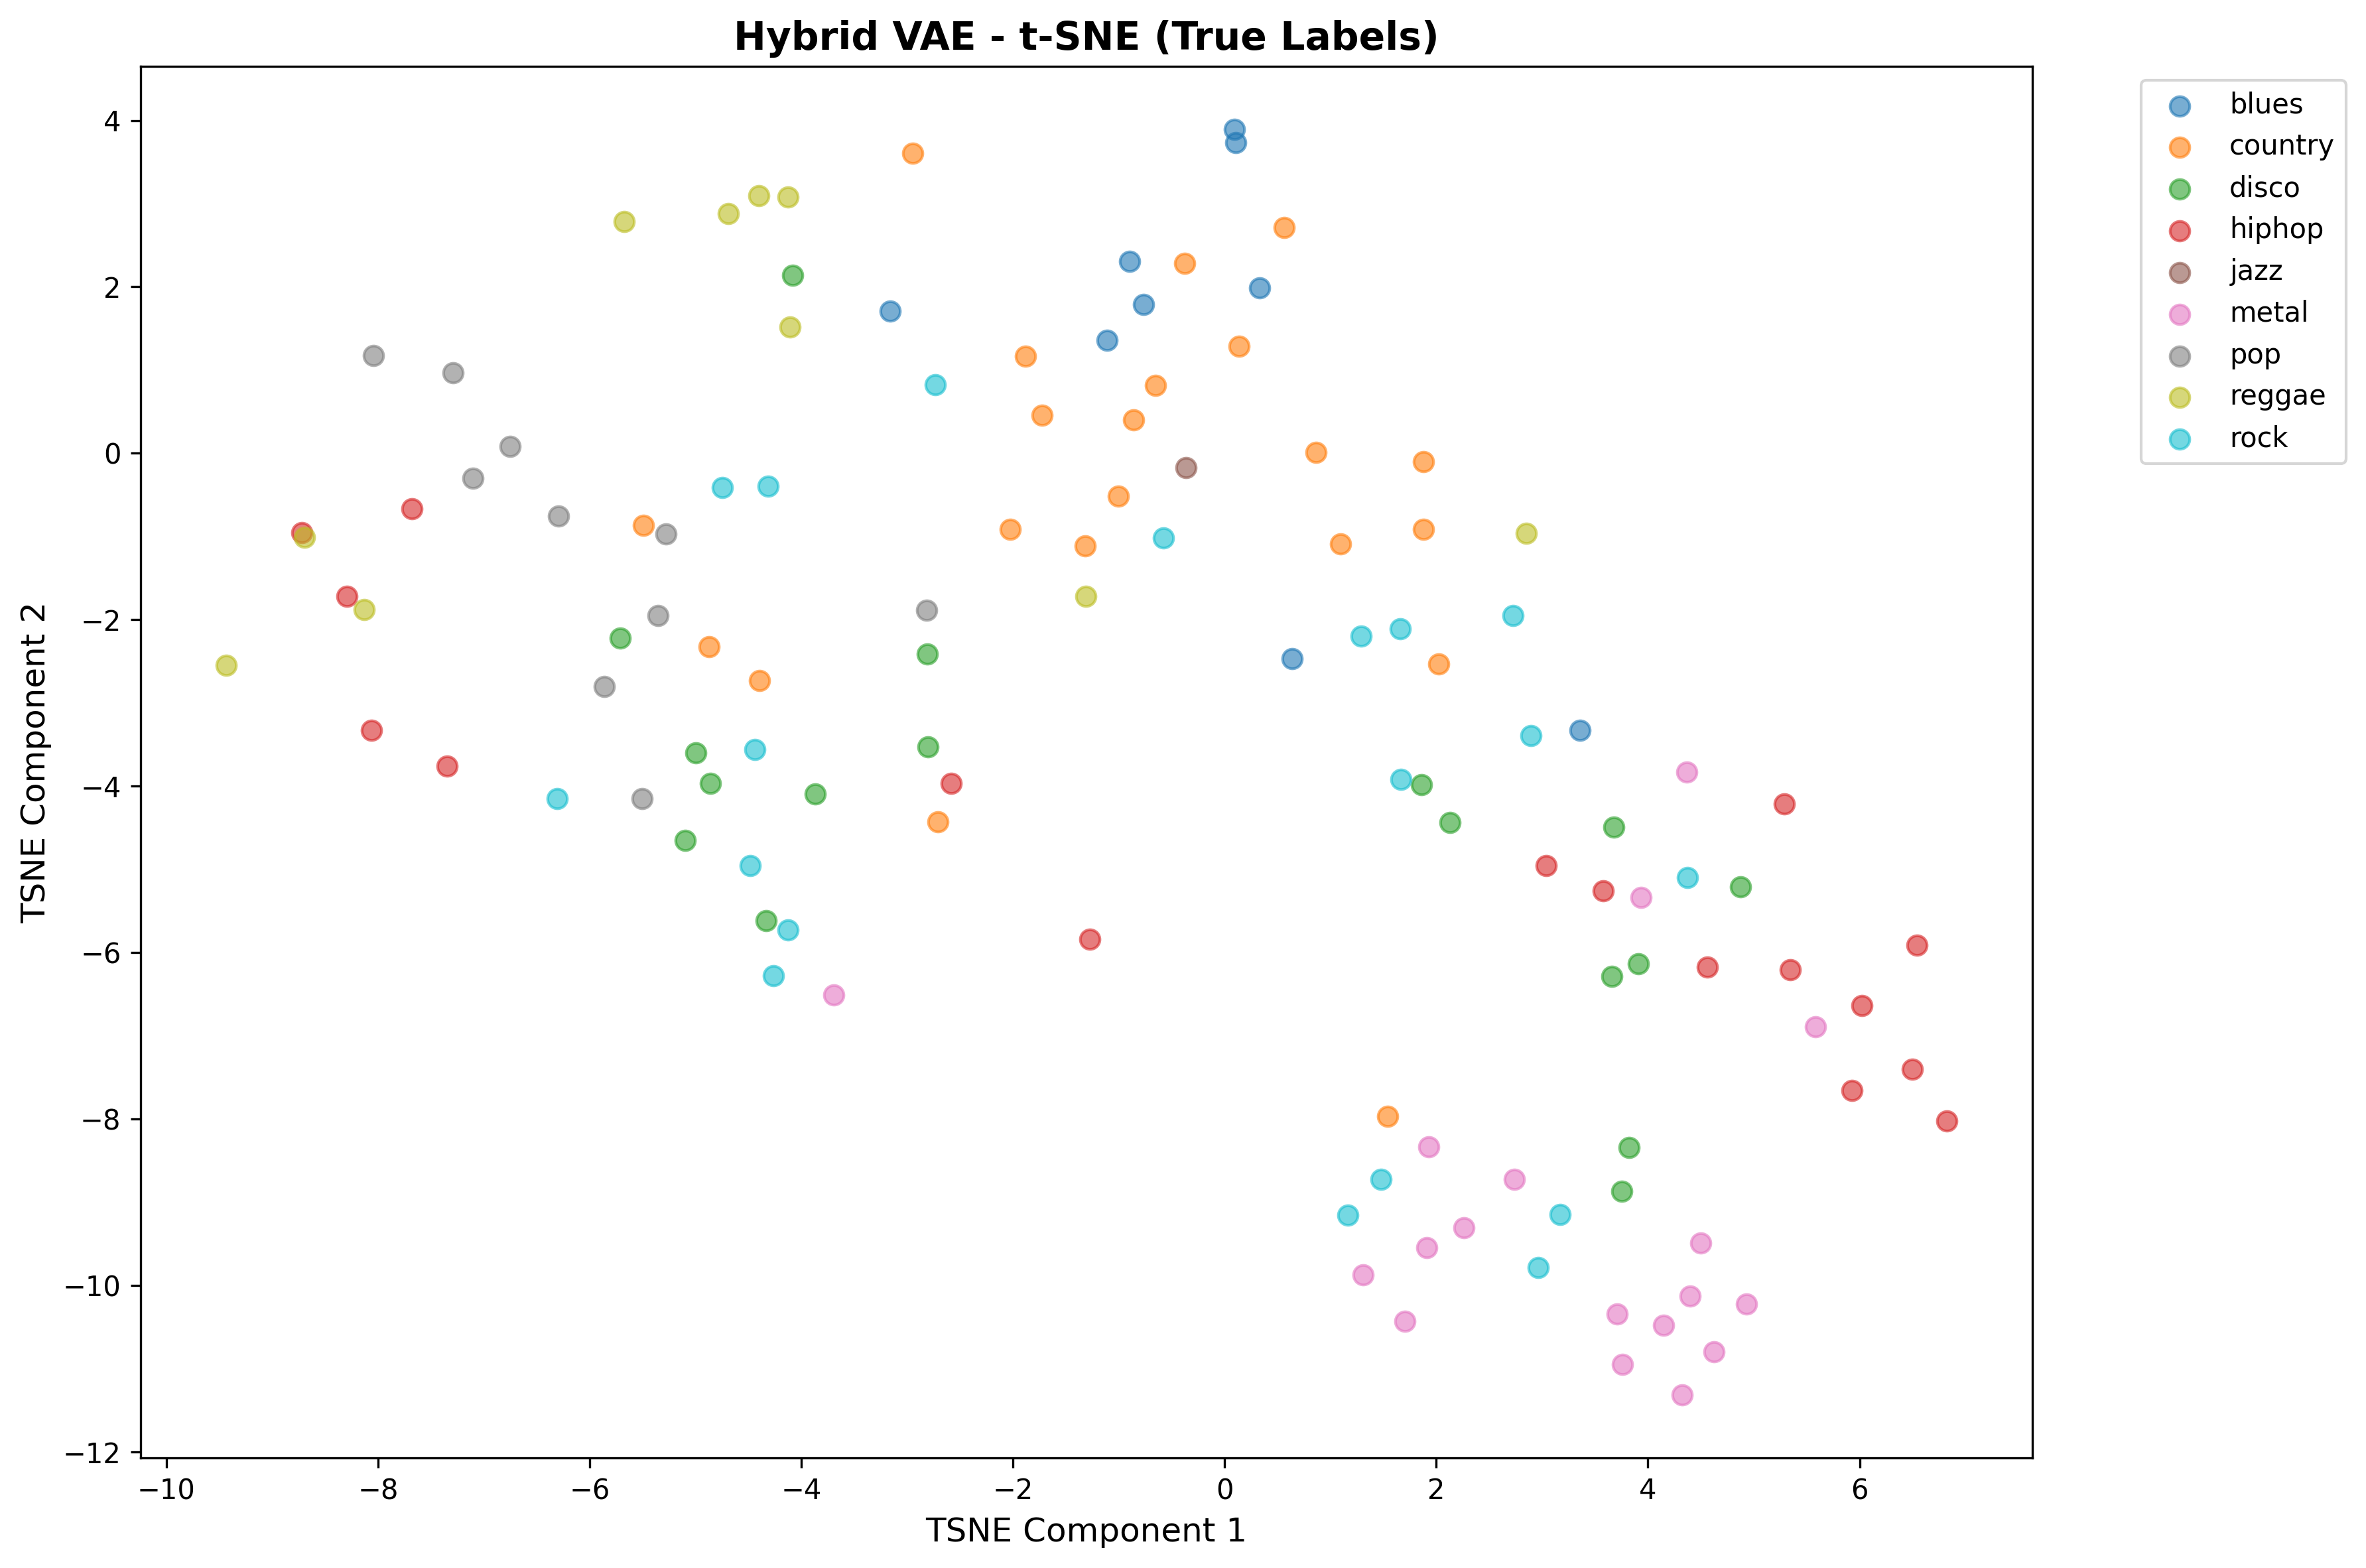
\includegraphics[width=0.9\linewidth]{../medium/results/hybrid_tsne_true.png}}{\fbox{Missing figure: ../medium/results/hybrid_tsne_true.png}}
\caption{HybridVAE latent space t-SNE (Medium).}
\end{figure}

\subsection{Hard: CVAE, Beta-VAE, and Baselines}
Metrics from \texttt{hard/results/comprehensive_comparison.csv} (selected methods).
\begin{table}[h]
\centering
\caption{Hard task comparison (selected methods).}
\begin{tabular}{lrrrrrr}
\toprule
Method & Sil. & CH & DB & ARI & NMI & Purity \\
\midrule
Beta-VAE ($\beta$=4.0) + K-Means & 0.1483 & 94.7497 & 0.9454 & 0.0679 & 0.2132 & 0.3689 \\
Beta-VAE ($\beta$=4.0) + Agglomerative & 0.1092 & 88.0715 & 1.1944 & 0.0415 & 0.2177 & 0.3197 \\
CVAE + K-Means & 0.0528 & 7.3974 & 1.9028 & 0.0171 & 0.1710 & 0.3033 \\
Autoencoder + K-Means & 0.0205 & 5.4361 & 1.9793 & 0.0616 & 0.2217 & 0.3689 \\
PCA + K-Means & 0.0081 & 4.8137 & 2.2755 & 0.0670 & 0.2296 & 0.3525 \\
\bottomrule
\end{tabular}
\end{table}

\begin{figure}[h]
\centering
\IfFileExists{../hard/results/comprehensive_comparison.png}{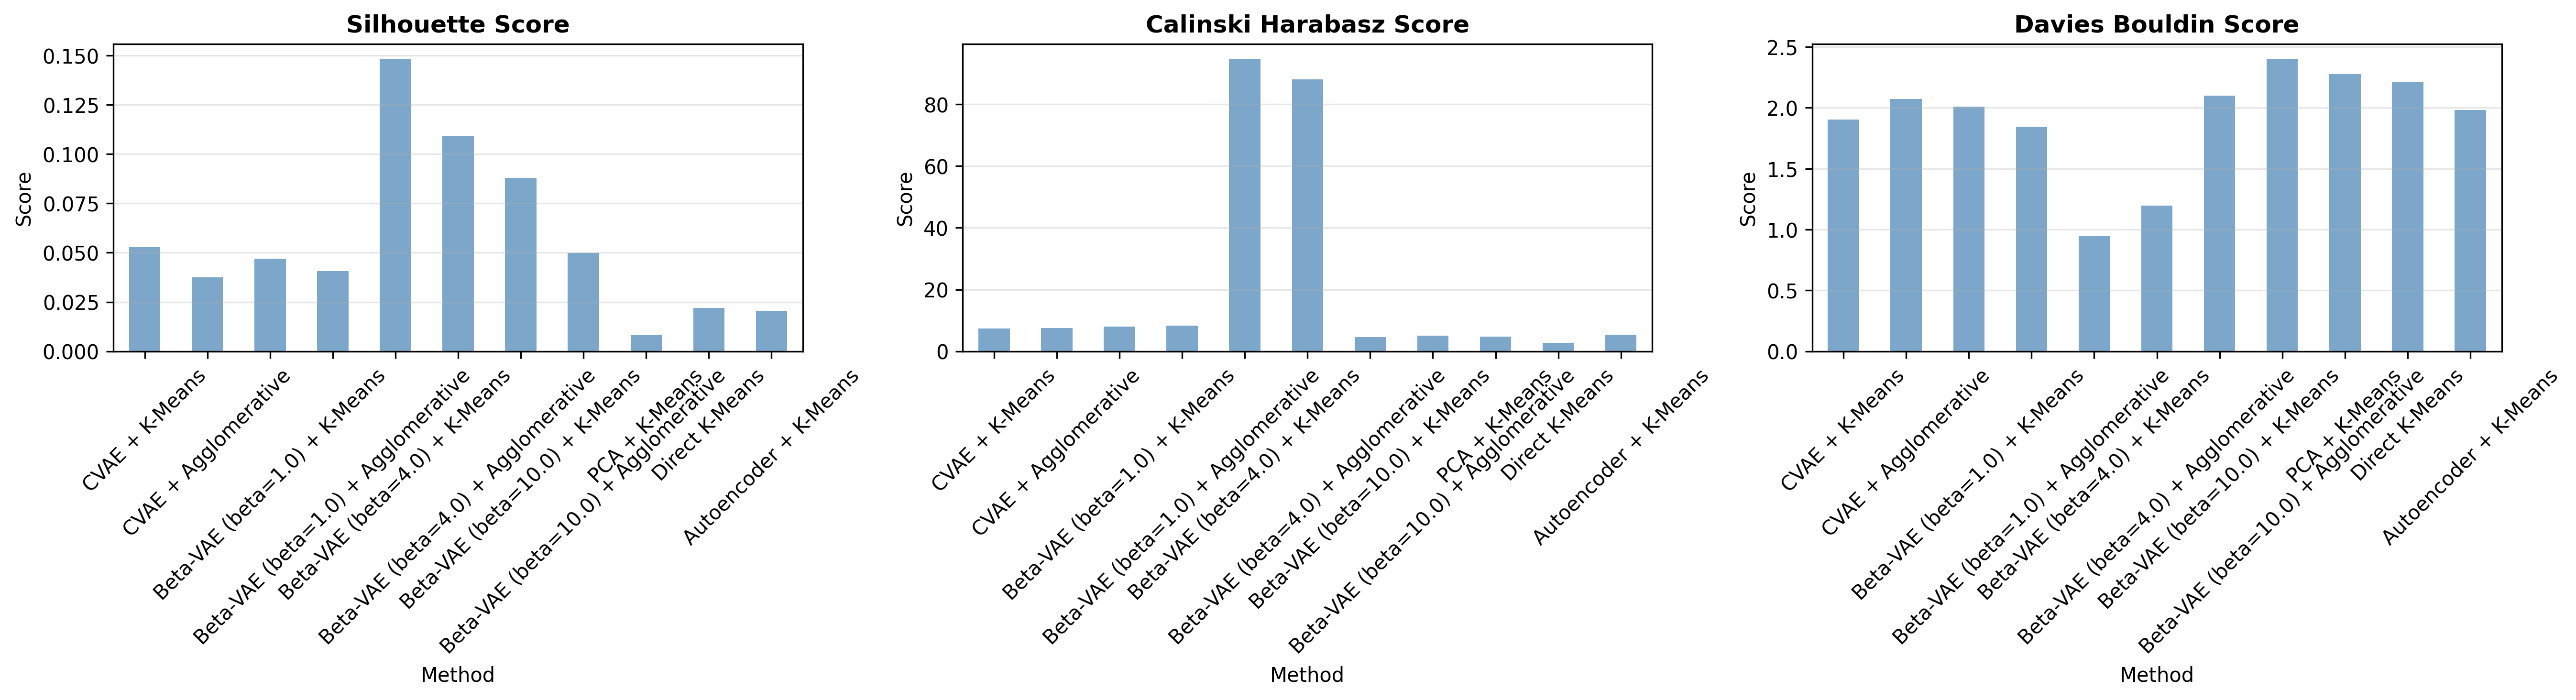
\includegraphics[width=0.9\linewidth]{../hard/results/comprehensive_comparison.png}}{\fbox{Missing figure: ../hard/results/comprehensive_comparison.png}}
\caption{Comprehensive comparison across methods (Hard).}
\end{figure}

\section{Discussion}
VAE latents improve clustering metrics over PCA, indicating non-linear embeddings capture genre-relevant structure from audio features. HybridVAE leverages lyrics to further increase Silhouette and NMI under Agglomerative/K-Means. In the hard setting, Beta-VAE with $\beta=4.0$ shows moderate latent separation but does not surpass hybrid clustering; CVAE conditioning yields modest gains, likely limited by sample size ($\sim$122) and modality mismatch.

\section{Conclusion}
Multi-modal VAEs provide promising improvements for genre clustering on GTZAN. HybridVAE offers the best overall balance in this project. Future work includes larger datasets, spectrogram-based ConvVAEs, improved lyric embeddings, and end-to-end multimodal training.

\section*{References}
\begin{thebibliography}{9}
\bibitem{kingma2014} Diederik P. Kingma and Max Welling. Auto-Encoding Variational Bayes. \emph{ICLR}, 2014.
\bibitem{higgins2017} Irina Higgins et al. beta-VAE: Learning Basic Visual Concepts with a Constrained Variational Framework. \emph{ICLR}, 2017.
\bibitem{sohn2015} Kihyuk Sohn, Honglak Lee, Xinchen Yan. Learning Structured Output Representation using Deep Conditional Generative Models. \emph{NIPS}, 2015.
\bibitem{gtzan} George Tzanetakis and Perry Cook. Musical genre classification of audio signals. \emph{IEEE TASLP}, 2002.
\bibitem{kmeans} Stuart Lloyd. Least squares quantization in PCM. \emph{IEEE}, 1982.
\end{thebibliography}

\end{document}
